\subsection{R-CNN}
\begin{frame}{}
    \LARGE Object Detection: \textbf{Regions with Convolutional Neural Networks (R-CNN)}
\end{frame}

\begin{frame}[allowframebreaks]{R-CNN}
    \begin{itemize}
        \item \textbf{R-CNN} stands for \textit{Regions with Convolutional Neural Networks}.
        \item Proposed by Ross Girshick et al. in 2014.
        \item Combines region proposals with CNNs for object detection.
        \item Steps:
        \begin{enumerate}
            \item Generate region proposals (e.g., using Selective Search).
            \item Warp each region and extract features using a CNN.
            \item Classify each region and refine bounding boxes.
        \end{enumerate}
        \item Achieved significant improvements over traditional methods (e.g., sliding windows, hand-crafted features).
    \end{itemize}

\framebreak

    \begin{figure}
        \centering
        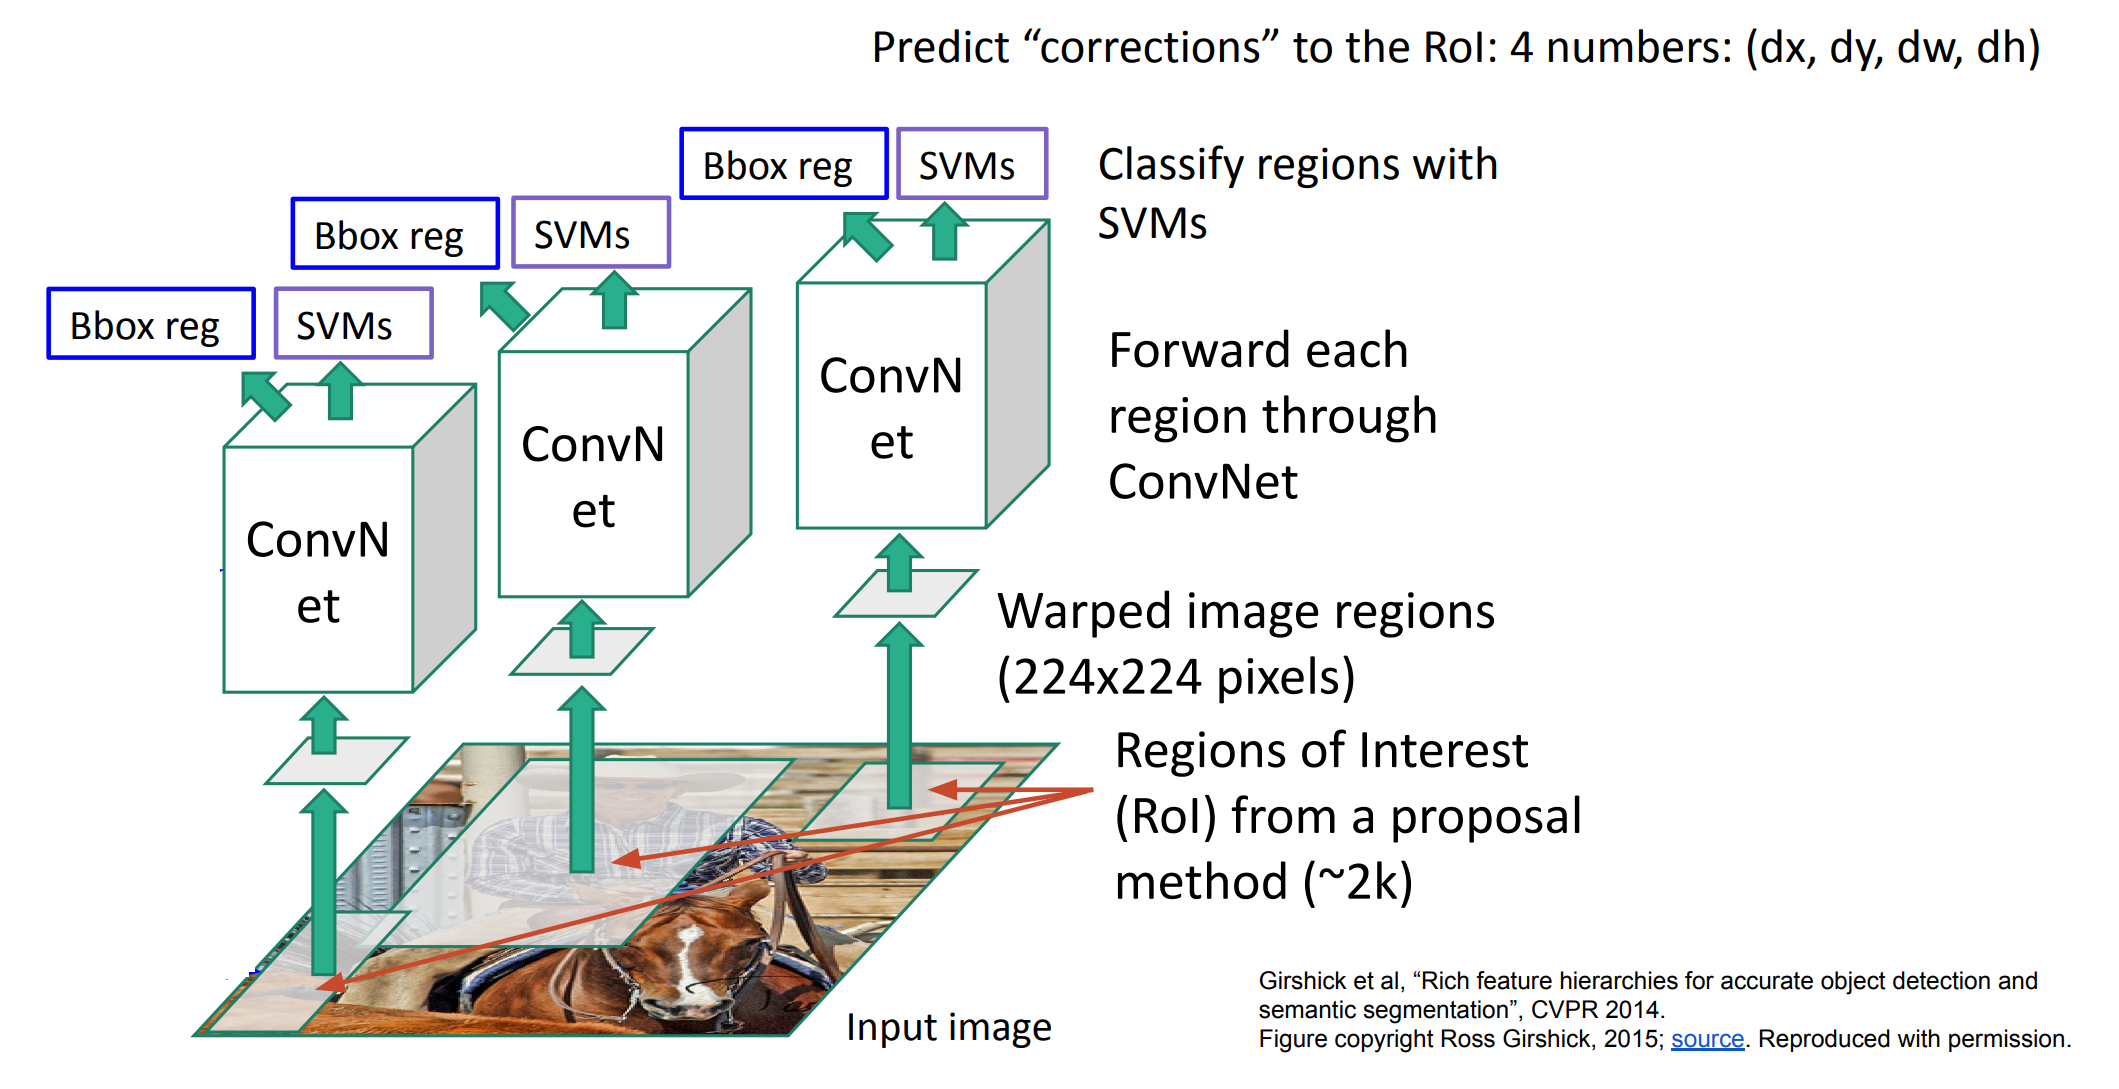
\includegraphics[width=1.0\textwidth,height=1.0\textheight,keepaspectratio]{images/object-detect/rcnn_1.png}
    \end{figure}

\framebreak

    \large R-CNN follows a \textbf{three-step pipeline} for object detection:
        \begin{enumerate}
            \item \textbf{Region Proposal (Selective Search)}
            \begin{itemize}
                \item Instead of using a brute-force sliding window approach, R-CNN applies \textbf{Selective Search}, an algorithm that identifies around \textbf{2000 candidate object regions} (called region proposals).
                \item This significantly reduces the number of regions to process, making the model more efficient.
            \end{itemize}
            \begin{figure}
                \centering
                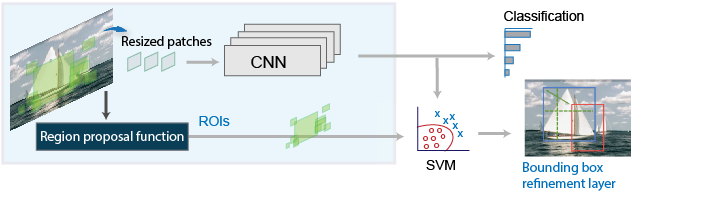
\includegraphics[width=1.0\textwidth,height=0.4\textheight,keepaspectratio]{images/object-detect/r-cnn-region-proposal.png}
            \end{figure}
\framebreak
            \item \textbf{Feature Extraction with CNN}
            \begin{itemize}
                \item Each region proposal is cropped from the image and resized to a fixed size (e.g., 224x224 pixels).
                \item The cropped regions are passed through a \textbf{pre-trained CNN} (like AlexNet or VGG16) to extract deep features.
                \item These features are then stored for classification.
            \end{itemize}
            \begin{figure}
                \centering
                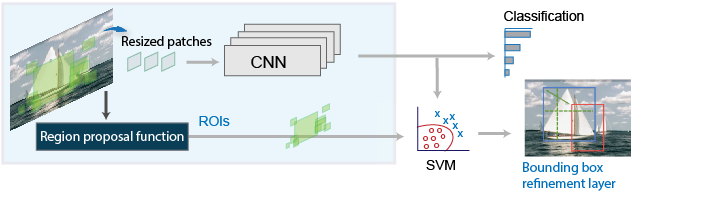
\includegraphics[width=1.0\textwidth,height=0.4\textheight,keepaspectratio]{images/object-detect/r-cnn-region-proposal.png}
            \end{figure}
\framebreak
            \item \textbf{Object Classification \& Bounding Box Refinement}
            \begin{itemize}
                \item The extracted features are passed through a \textbf{Support Vector Machine} (SVM) classifier to determine the object category.
                \item A \textbf{bounding box regression} model is used to fine-tune the position of the detected objects.
            \end{itemize}
            \begin{figure}
                \centering
                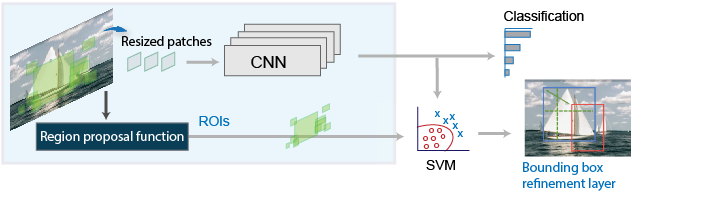
\includegraphics[width=1.0\textwidth,height=0.4\textheight,keepaspectratio]{images/object-detect/r-cnn-region-proposal.png}
            \end{figure}
        \end{enumerate}

\framebreak

        \begin{figure}
            \centering
            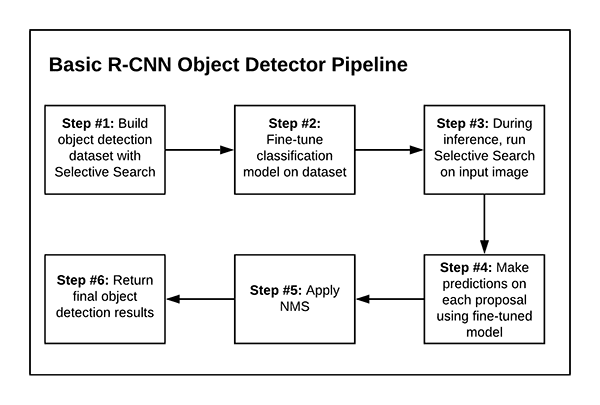
\includegraphics[width=1.0\textwidth,height=0.9\textheight,keepaspectratio]{images/object-detect/r-cnn-pipeline.png}
        \end{figure}
\end{frame}

\begin{frame}[allowframebreaks]{R-CNN: Problem}
    \begin{figure}
        \centering
        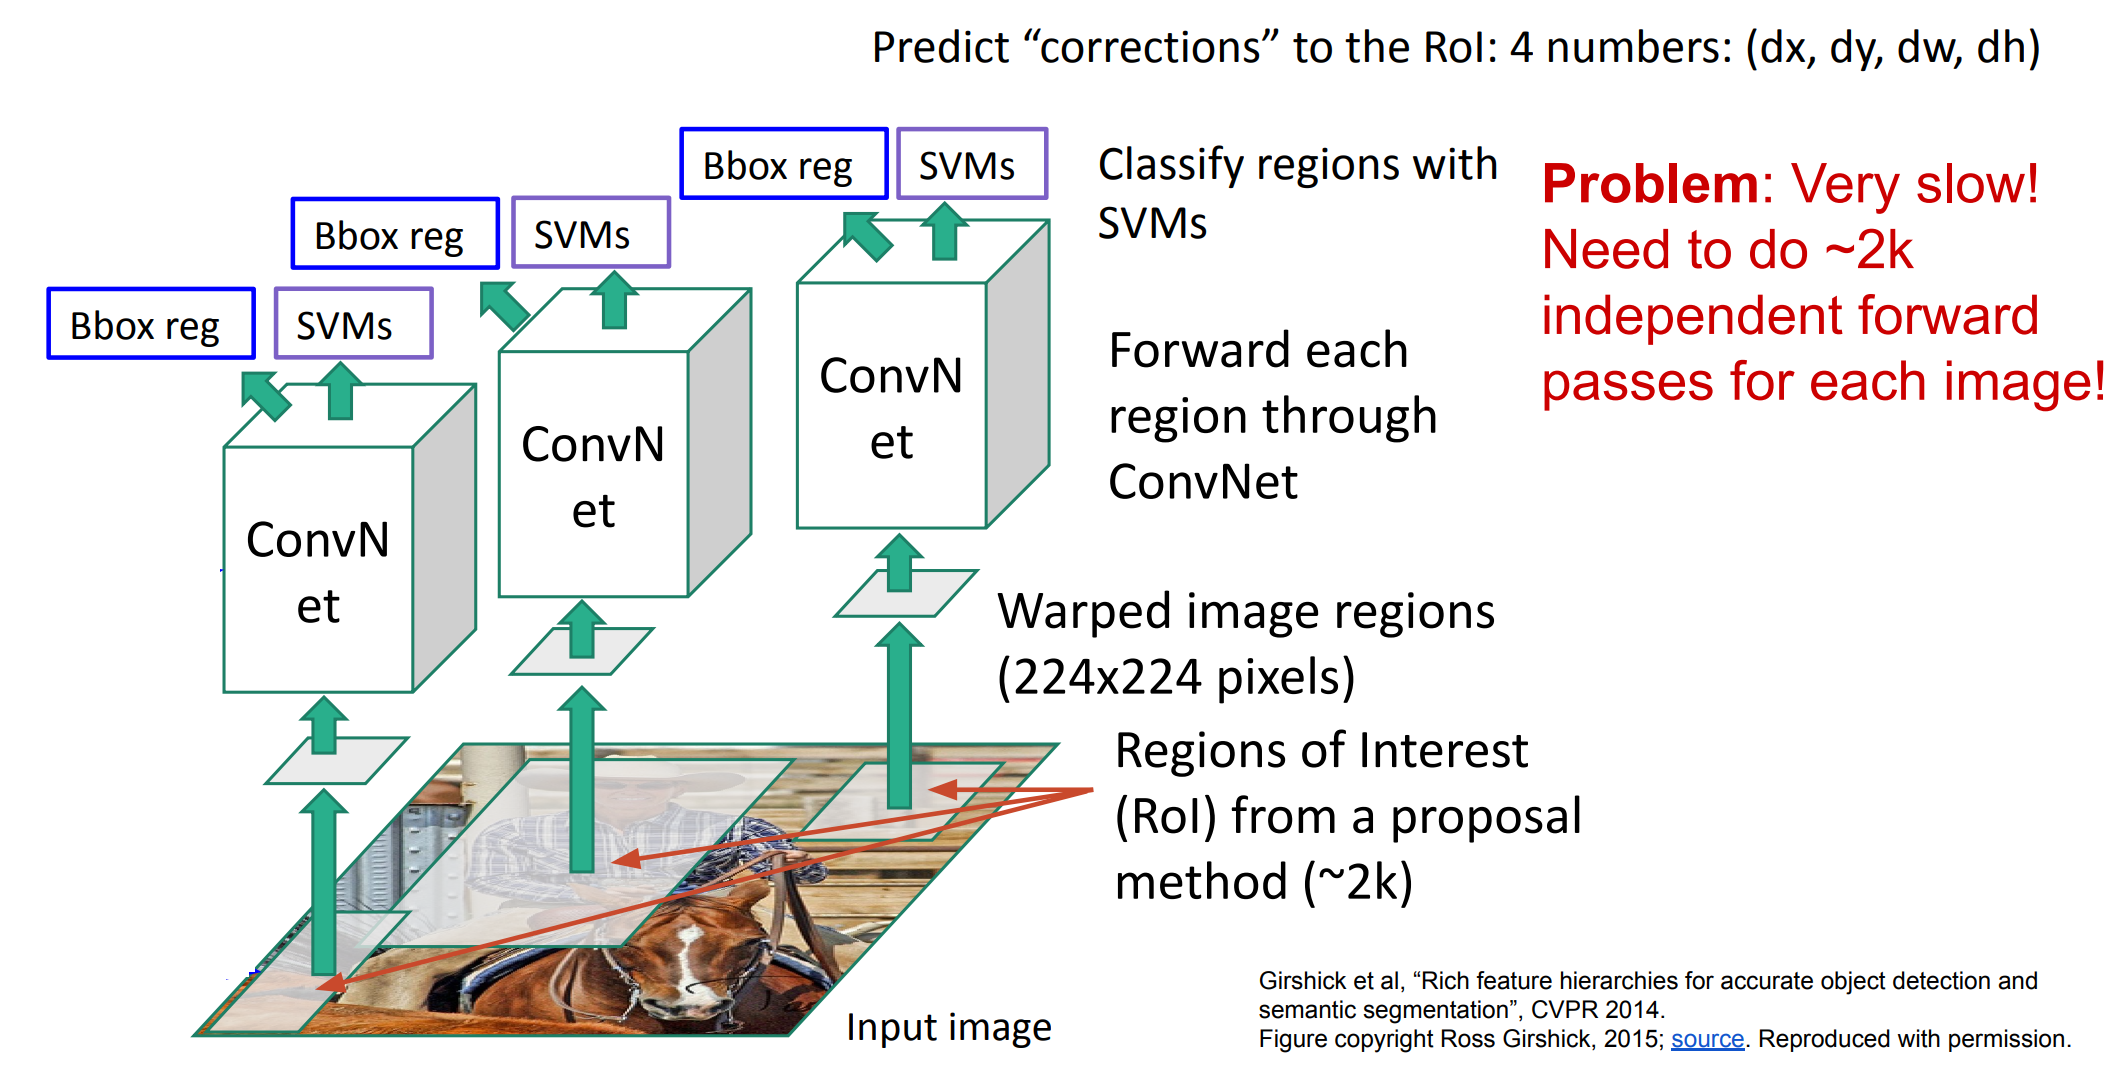
\includegraphics[width=1.0\textwidth,height=1.0\textheight,keepaspectratio]{images/object-detect/rcnn_2.png}
    \end{figure}

\framebreak

    \begin{figure}
        \centering
        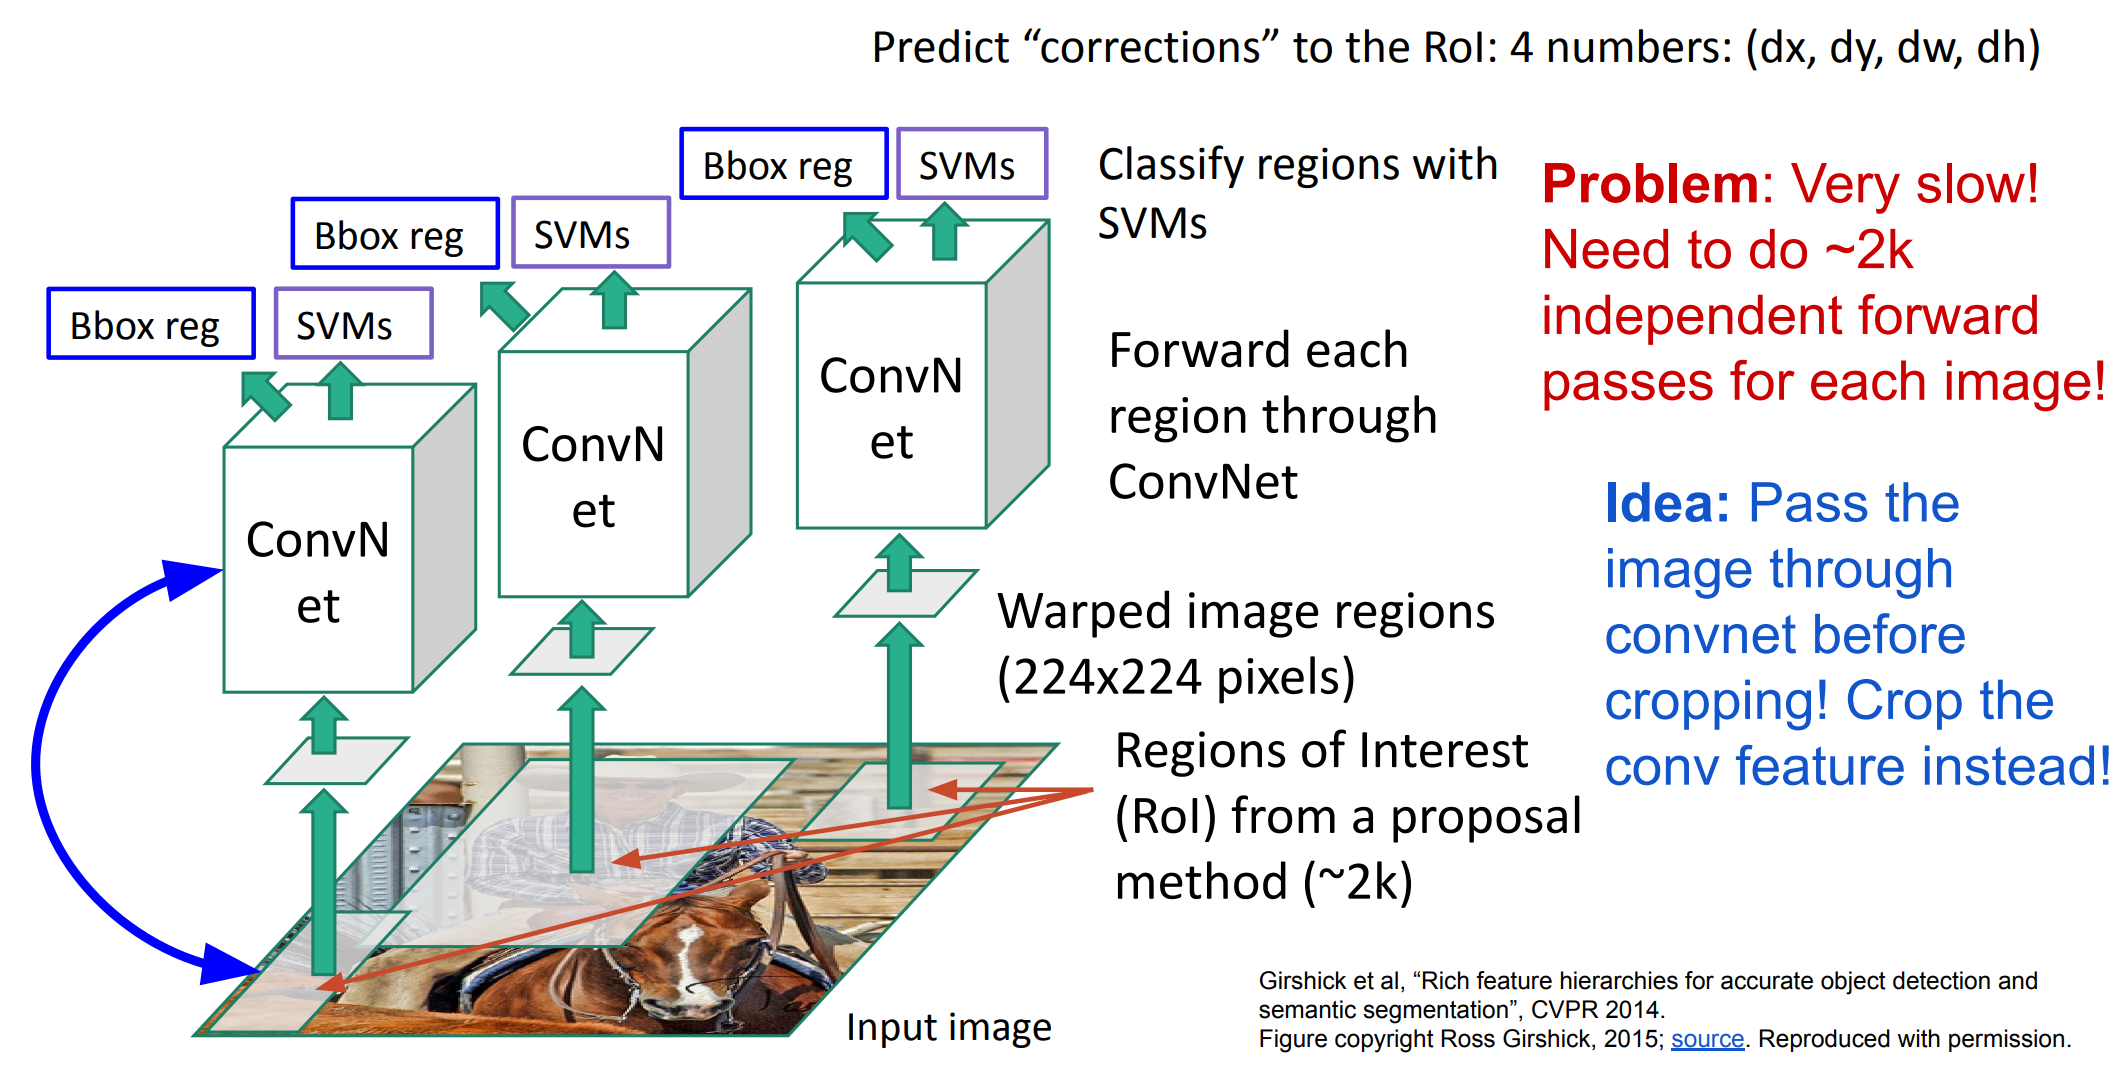
\includegraphics[width=1.0\textwidth,height=1.0\textheight,keepaspectratio]{images/object-detect/rcnn_3.png}
    \end{figure}
\end{frame}

\begin{frame}{Evolution of R-CNN}
    \begin{itemize}
        \item \textbf{R-CNN} inspired a series of improved models:
        \begin{itemize}
            \item \textbf{Fast R-CNN}: Performs feature extraction for all region proposals in a single forward pass, greatly increasing speed and efficiency.
            \item \textbf{Faster R-CNN}: Introduces a \textbf{Region Proposal Network (RPN)} to generate region proposals, making the process end-to-end and even faster.
            \item \textbf{Mask R-CNN}: Extends Faster R-CNN by adding a branch for predicting segmentation masks, enabling instance segmentation.
        \end{itemize}
        \item These advancements have made deep learning-based object detection both faster and more accurate.
    \end{itemize}
\end{frame}